\subsection{Audio-Schaltung}
\label{subsec:Audio-Schaltung}

Für die Validierung des Analog-Teils wurden verschiedene Teil-Messungen durchgeführt welche nachfolgend erklärt werden.

\subsubsection{Frequenzgang}
\label{subsubsec:Frequenzgang}
Um zu beurteilen ob die Audio-Wandlung und Rückwandlung korrekt funktioniert wird der Frequenzgang der entworfenen Schaltung gemessen. Damit sollte ersichtlich werden welche Frequenz mit welcher Verstärkung von Ein- zu Ausgang übertragen wird. Angestrebt wäre eine möglichst linearer Frequenzgang mit einer Verstärkung von 1 (0dB) auf allen Frequenzen.

\textbf{Anmerkung:} Da am Line-Eingang ein Spannungsteiler die Amplitude des Signals halbiert wurde dies software-mässig korrigiert. Das heisst 0dB in der Software bewirkt eigentlich +6dB am Codec, aber wiederum 0dB auf die ganze Schaltung gesehen wegen des Spannungsteilers.

\begin{figure} [H]
\begin{center}
 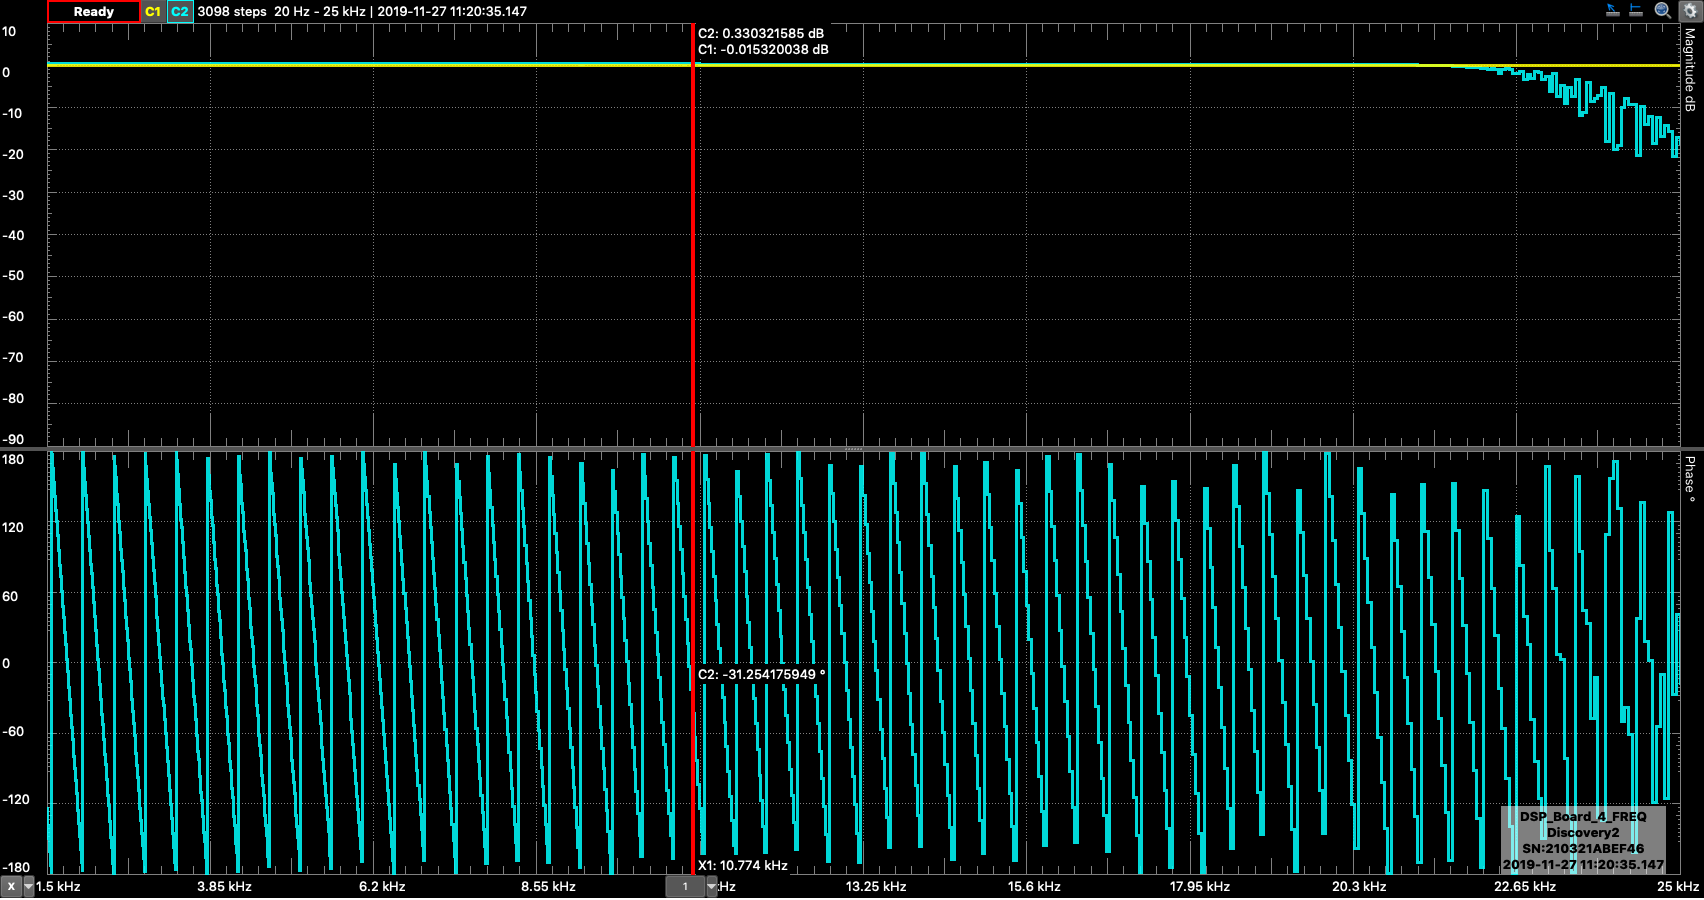
\includegraphics[scale=0.23]{../graphics/DSP_Board_FREQ.png}
 \caption{Der gemessene Frequenzgang von Audio-Eingang zu Audio-Ausgang (oben) sowie der Phasengang der Schaltung(unten)}
\label{fig:frequenzgang}
\end{center}
\end{figure}
\todo{Frequenzgang nochmal messen}
Die Messung wurde mit einem Analog Discovery 2 von Digilent durchgeführt. In Gelb wurde das Referenz-Signal gemessen und in Blau die Antwort durch die Schaltung. Wie zu erwarten fängt das Anti-Aliasing-Filter bei der halben Abtastfrequenz (22.05kHz) an zu sperren. Der Phasengang ist wie erwartet linear mit entsprechenden Wrap-around von -180° zu 180°.

\subsubsection{Total Harmonic Distortion}
\label{subsubsec:Total Harmonic Distortion}
Die Total Harmonic Distortion oder auch THD genannt ist ein Leistungs-Verhältnis der harmonischen Oberschwingungen zum ursprünglich  eingespeisten Signal. In diesem Fall ist das eine Sinusschwingung mit einer Frequenz von 1kHz und $1V_{PP}$ Amplitude. Mit dem Stanford SR770 FFT Network Analyzer kann die THD direkt gemessen werden.

\begin{figure} [H]
\begin{center}
 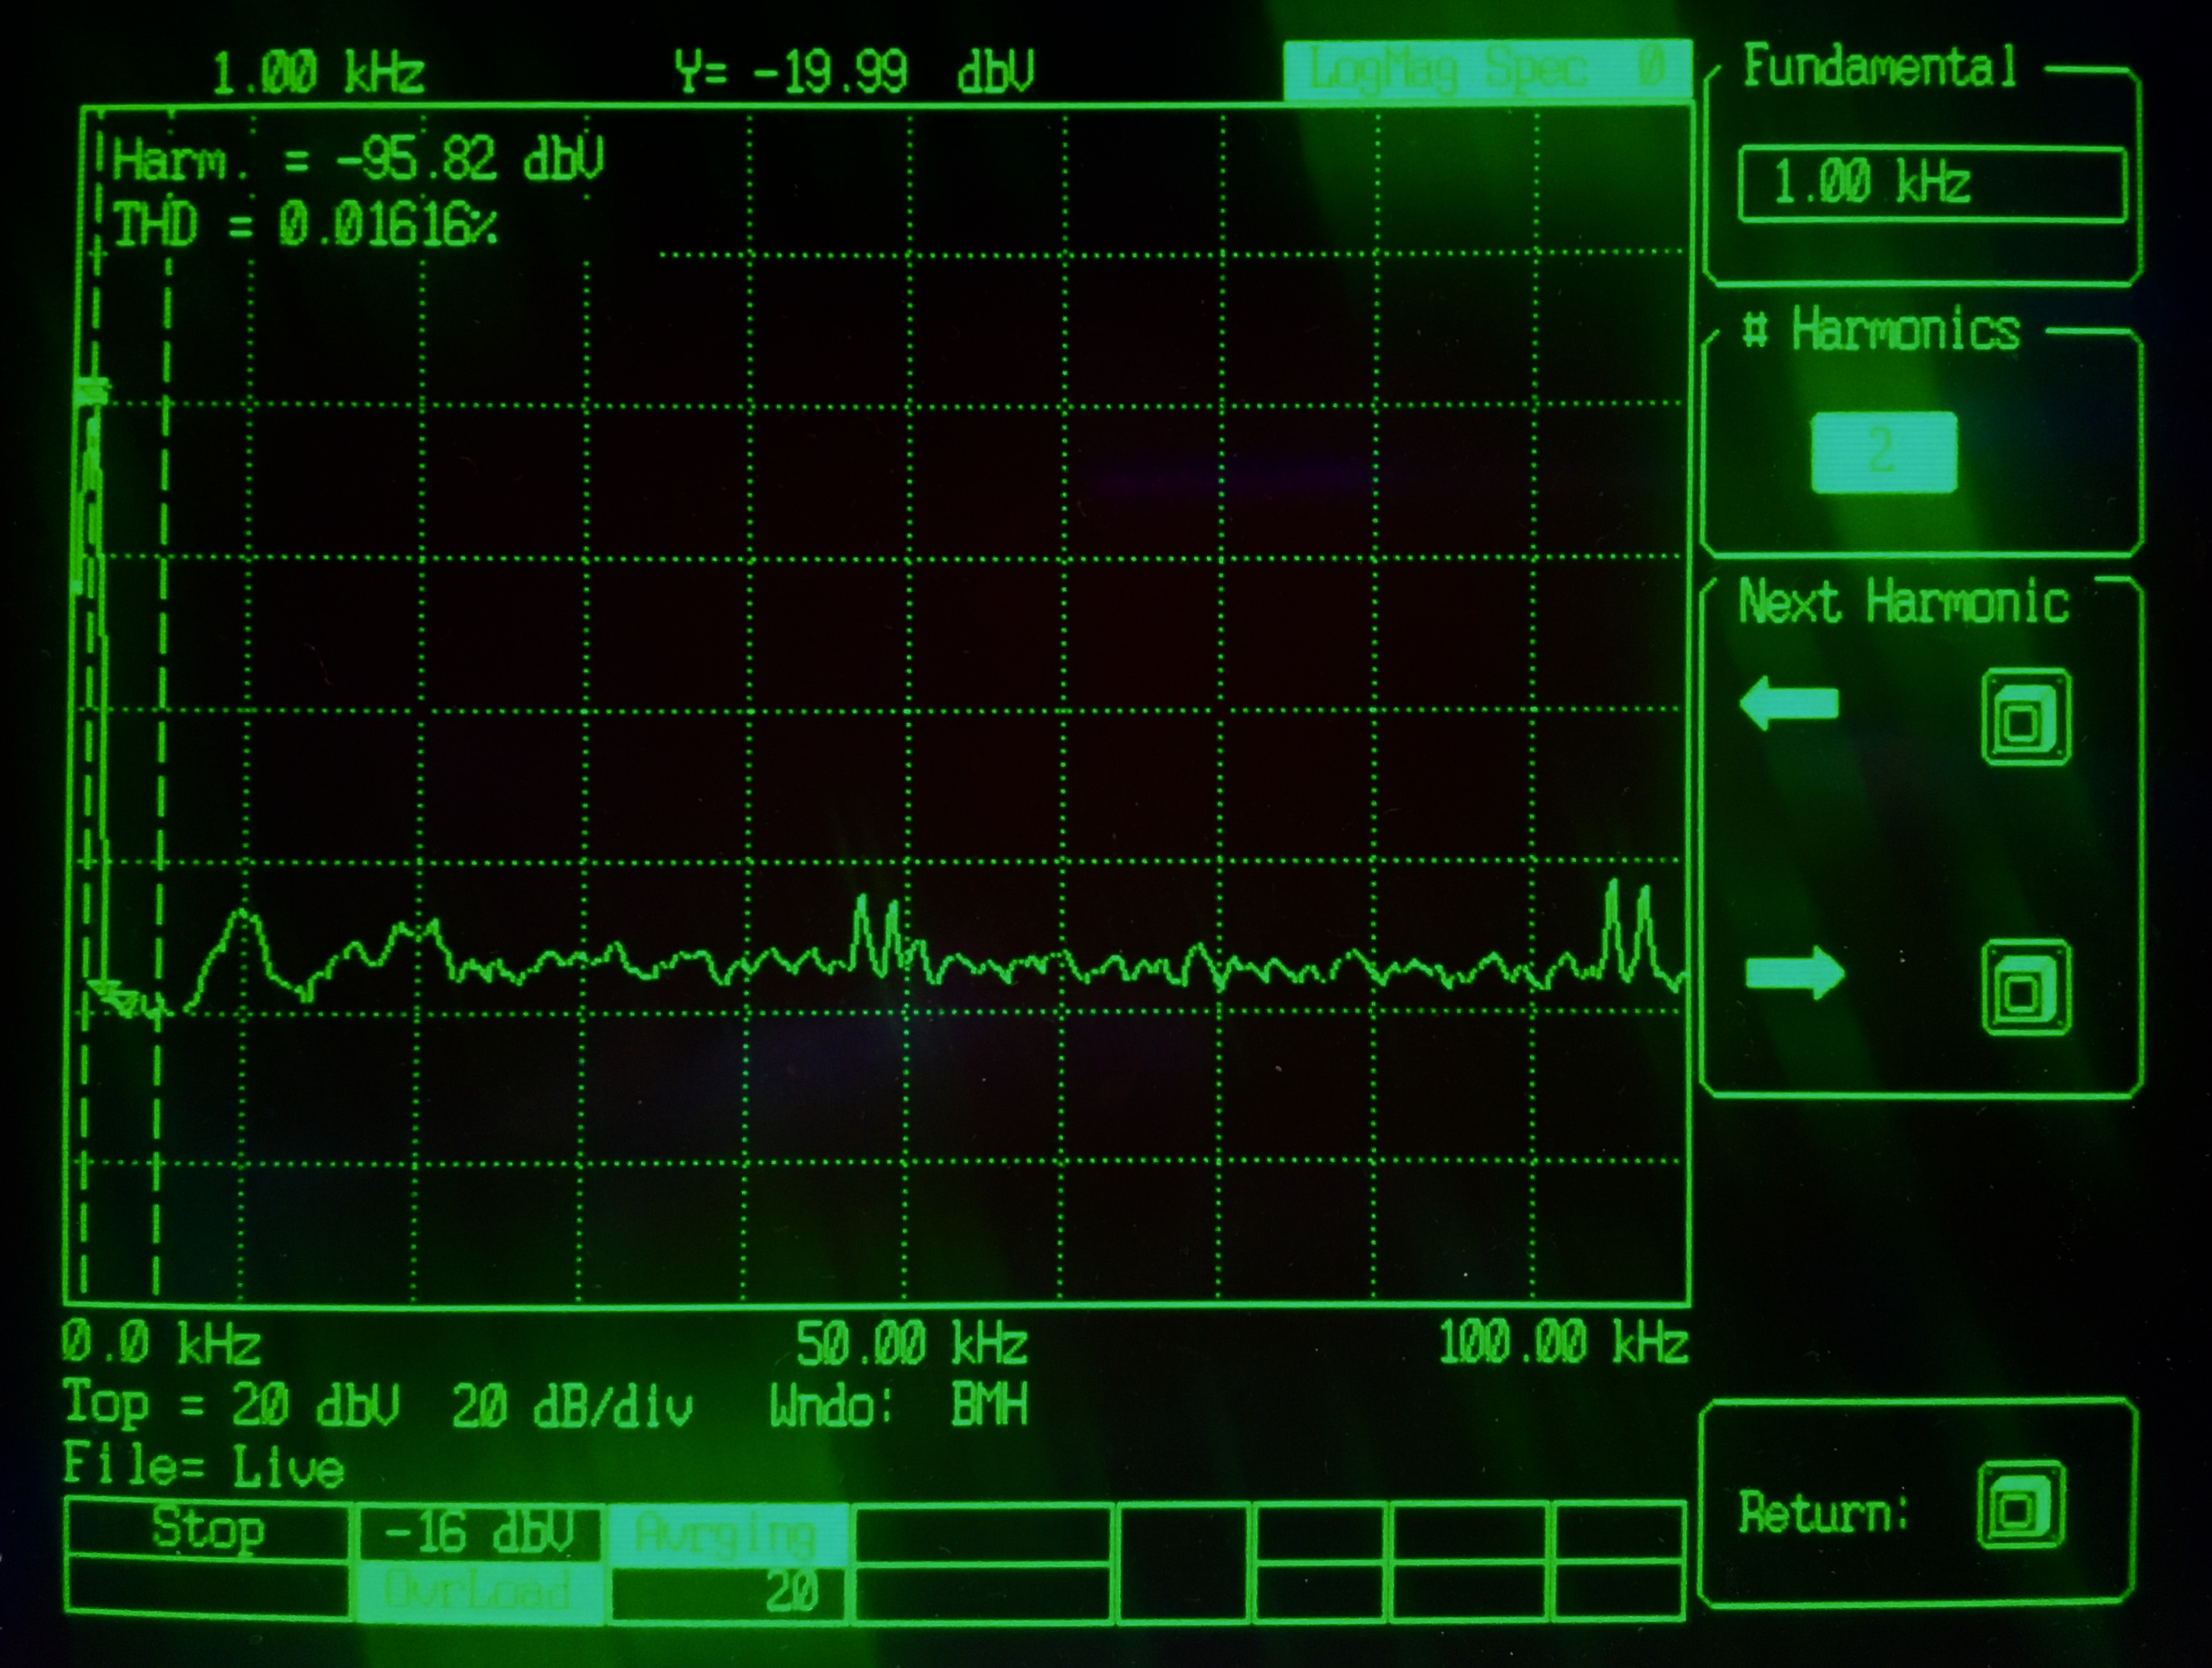
\includegraphics[scale=0.1]{../graphics/THD.jpg}
 \caption{Die gemessene Total Harmonic Distortion}
\label{fig:frequenzgang}
\end{center}
\end{figure}